\documentclass{article}
\usepackage[utf8]{inputenc}
\usepackage[T1]{fontenc}
\usepackage[letterpaper, margin=2cm]{geometry}
\usepackage{dingbat}
\usepackage{amsmath, amsthm, amsfonts, amssymb}
\usepackage{mathtools}
\usepackage{enumitem}
\usepackage[dvipsnames]{xcolor}
\usepackage{tikz}
\usepackage[framemethod=tikz]{mdframed}
\usepackage{array}
\usepackage{epigraph}
\usepackage{wasysym}
\usepackage{hyperref}


\usetikzlibrary{decorations.pathmorphing}

\setlength{\parindent}{0.25cm}
\setlist[description]{leftmargin=0.5cm, style=nextline, noitemsep, topsep=0.25pt}
\setlist[itemize]{style=nextline, itemsep=0.25pt, topsep=0.25pt, label={$\Rightarrow$}}

\hypersetup{
    colorlinks,
    linkcolor={red!50!black},
    citecolor={blue!50!black},
    urlcolor={blue!80!black}
}

\allowdisplaybreaks

\newtheoremstyle{customstyle}%            % Name
  {}%                                     % Space above
  {}%                                     % Space below
  {}%                                     % Body font
  {}%                                     % Indent amount
  {\bfseries}%                            % Theorem head font
  {.}%                                    % Punctuation after theorem head
  { }%                                    % Space after theorem head, ' ', or \newline
  {\thmname{#1}\thmnumber{ #2}\thmnote{ (#3)}}%
\theoremstyle{customstyle}

\newmdtheoremenv[innertopmargin=-2pt, skipbelow=0pt, linewidth=2pt, linecolor=Green, backgroundcolor=Green!10, bottomline=false, leftline=false, rightline=false]{theorem}{Theorem}

\makeatletter
\g@addto@macro\bfseries{\boldmath}
\makeatother

\newcommand{\NTIME}{\ensuremath{\textsf{NTIME}}}
\newcommand{\coNTIME}{\ensuremath{\textsf{coNTIME}}}
\newcommand{\Poly}{\ensuremath{\textsf{P}}}
\newcommand{\EXP}{\ensuremath{\textsf{EXP}}}
\newcommand{\NP}{\ensuremath{\textsf{NP}}}
\newcommand{\NEXP}{\ensuremath{\textsf{NEXP}}}
\newcommand{\NEXPEXP}{\ensuremath{\textsf{NEXPEXP}}}
\newcommand{\coNP}{\ensuremath{\textsf{coNP}}}
\newcommand{\coNEXP}{\ensuremath{\textsf{coNEXP}}}
\newcommand{\coNEXPEXP}{\ensuremath{\textsf{coNEXPEXP}}}
\newcommand{\interP}{\ensuremath{\textsf{NP}\cap\textsf{coNP}}}
\newcommand{\interEXP}{\ensuremath{\textsf{NEXP}\cap\textsf{coNEXP}}}
\newcommand{\interEXPEXP}{\ensuremath{\textsf{NEXPEXP}\cap\textsf{coNEXPEXP}}}
\newcommand{\unionP}{\ensuremath{\textsf{NP}\cup\textsf{coNP}}}
\newcommand{\unionEXP}{\ensuremath{\textsf{NEXP}\cup\textsf{coNEXP}}}
\newcommand{\unionEXPEXP}{\ensuremath{\textsf{NEXPEXP}\cup\textsf{coNEXPEXP}}}
\newcommand{\tup}{\text{\rightthumbsup}}
\newcommand{\tdown}{\text{\rightthumbsdown}}

% zigzag arrows
\newlength{\LETTERheight}
\AtBeginDocument{\settoheight{\LETTERheight}{I}}
\newcommand*{\longleadsto}[1]{\ \raisebox{0.24\LETTERheight}{\tikz \draw [->,
line join=round,
decorate, decoration={
    zigzag,
    segment length=4,
    amplitude=.9,
    post=lineto,
    post length=2pt
}] (0,0) -- (#1,0);}\ }

% thick lines in the Bingo card
\makeatletter
\newcommand{\thickhline}{%
    \noalign {\ifnum 0=`}\fi \hrule height 1pt
    \futurelet \reserved@a \@xhline
}
\newcolumntype{"}{@{\hskip\tabcolsep\vrule width 1pt\hskip\tabcolsep}}
\makeatother

\renewcommand\thetheorem{\Roman{theorem}}

\newcounter{exercise}
\newenvironment{exercise}[1][]{\refstepcounter{exercise}\par\medskip\noindent\textbf{Exercise~\theexercise.#1} \rmfamily}{\medskip}

\begin{document}

\title{The Nondeterministic Time Hierarchy}
\author{Sebastian Oberhoff\\{\small oberhoff.sebastian@gmail.com}}
\date{\today}

\maketitle

\begin{abstract}
\begin{center}
Let's play some Bingo. Here's our card:\medskip

\begin{tabular}{|c"c|c|c|c|}
\hline
& \NEXP & \coNEXP & \interEXP & \unionEXP\\\thickhline
\NP & & & & \\\hline
\coNP & & & & \\\hline
\interP & & & & \\\hline
\unionP & & & & \\\hline
\end{tabular}\medskip

Using simple brute force all the classes on the left are contained in those at the top. But are these containments strict? That's the challenge: to put a ``$\subsetneq$'' in every spot. Hold on to your potatoes.
\end{center}
\end{abstract}

\setlength{\epigraphwidth}{\textwidth}

\epigraph{I find that if I just sit down and think... the solution presents itself.}{\textit{Professor Henry Jones Sr.}}

\begin{figure}[h]
\centering
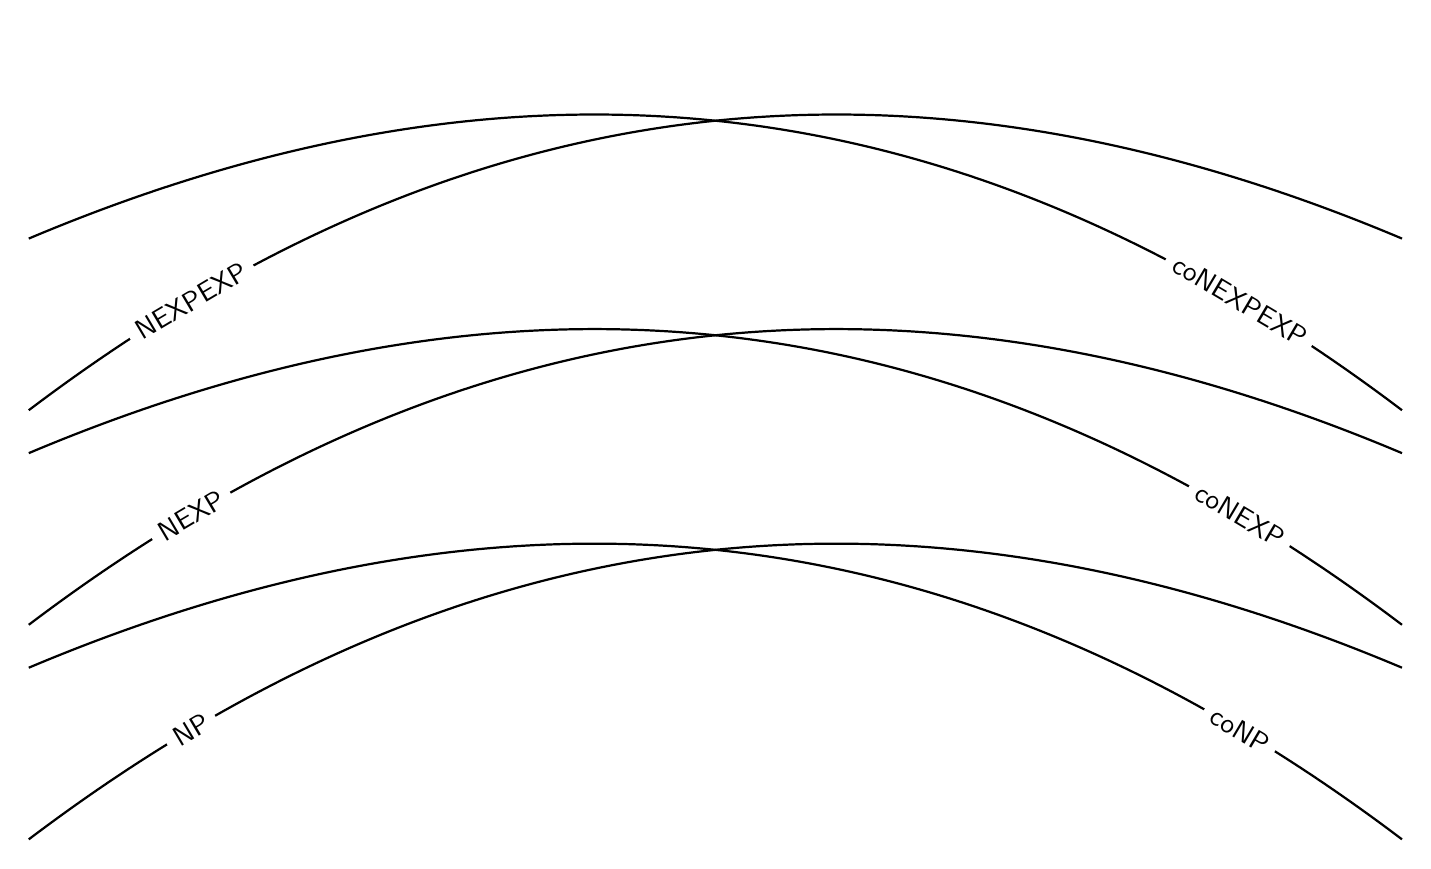
\begin{tikzpicture}[scale=1.09]
\draw[thick] (-8, 0) to[bend left] node[very near start, sloped, fill=white] {$\NP$} (8, 2);
\draw[thick] (8, 0) to[bend right] node[very near start, sloped, fill=white] {$\coNP$} (-8, 2);
\draw[thick] (-8, 2.5) to[bend left] node[very near start, sloped, fill=white] {$\NEXP$} (8, 4.5);
\draw[thick] (8, 2.5) to[bend right] node[very near start, sloped, fill=white] {$\coNEXP$} (-8, 4.5);
\draw[thick] (-8, 5) to[bend left] node[very near start, sloped, fill=white] {$\NEXPEXP$} (8, 7);
\draw[thick] (8, 5) to[bend right] node[very near start, sloped, fill=white] {$\coNEXPEXP$} (-8, 7);
\end{tikzpicture}
\caption{The Nondeterministic Time Hierarchy.}
\label{figure}
\end{figure}

\section{``Se\~{n}or, Nobody's Come Out Of There Alive.''}

\begin{theorem}
$\NP \subsetneq \NEXP$.\label{NDTH}
\end{theorem}

\begin{proof}
Let's start by contemplating the following problem:
\begin{mdframed}
\textsc{NCatch22}$^n$

\noindent
$
\hspace{-1pt}
\left.\parbox{0.4\textwidth}{
\begin{itemize}[noitemsep,topsep=0.3em]
\item[$\longrightarrow$] A nondeterministic algorithm $N$.
\item[$\longrightarrow$] An integer $t$ in \textit{unary}.
\end{itemize}
}\right\}\;
\text{$n$ bits in total.}\hspace*{\fill}
$
\begin{itemize}[noitemsep,topsep=0.3em]
\item[$\longleftarrow$] Accept if there's no path of execution such that $N(N, t)$ accepts within $2^n$ steps. Reject otherwise.
\end{itemize}
\end{mdframed}
On the one hand, we can solve this problem in deterministic doubly exponential time by just going through all possible lines of execution. This is true even if $N$ varies, not just $t$. Increasing the size of the source code of $N$ isn't \textit{that} catastrophic. So if we give ourselves an expexporbitant budget, we're good. That puts the problem in \textsf{EXPEXP} and thereby in $\NEXPEXP$.

On the other hand, suppose for a moment that we could somehow solve this problem in $f(n) \in o(2^n)$ steps with some nondeterministic algorithm $N^*$. Any such algorithm could be turned back around on itself by asking whether there exists a path of execution such that $N^*(N^*, t)$ accepts within $2^n$ steps. Let $t$ be large enough so that $f(n) \ll 2^n$, then:\\[0.5em]
\begin{minipage}{0.4\textwidth}
\begin{description}
\item[Either there is such a path:]
\begin{itemize}
\item[]
\item $N^*(N^*, t)$ always rejects.
\item There is no such a path. \lightning
\end{itemize}
\end{description}
\end{minipage}
\begin{minipage}{0.55\textwidth}
\begin{description}
\item[Or there is no such path:]
\begin{itemize}
\item[]
\item $N^*(N^*, t)$ \textit{someway} accepts within $f(n)$ steps.
\item There is such a path. \lightning
\end{itemize}
\end{description}
\end{minipage}\\[1em]
As we can see, it's impossible for any nondeterministic algorithm to accomplish this task in $o(2^n)$ steps. In particular, because $O\bigl(2^{n/2}\bigr) \subseteq o(2^n)$, it's impossible to accomplish this task in $\NTIME\bigl(2^{n/2}\bigr)$. And since this class contains all of nondeterministic polynomial time we have
\[
\NP \subseteq \NTIME\bigl(2^{n/2}\bigr) \subsetneq \NEXPEXP\,.
\]
Just one small problem. That's one ``\textsf{EXP}'' too many. Dang it!

At this point the classical route is to start over and try something cleverer instead: lazy diagonalization~\cite{stanislav}. Certainly, that's the way to go if you want to squeeze out the best possible Nondeterministic Time Hierarchy Theorem. But we're not here for elaborately choreographed sword fights. We're here to cleave the polynomial and the exponential apart. So let's just shoot the sucker.

Imagine $\NP = \NEXP$. Then $\NEXP = \NEXPEXP$. How so? \textit{Padding}, that's how. Therefore, by chaining our equalities we get $\NP = \NEXP = \NEXPEXP$. And \textit{that} we know isn't true. QED.\footnote{Out of curiosity I asked Stephen Cook, who first established the strong form of the Nondeterministic Time Hierarchy in 1972~\cite{cook}, whether he already knew this argument at the time. The answer appears to be ``no''. Though he can't be sure anymore.}

All that's left over is to double check the details involved in the padding. For this take any problem in $\NEXPEXP$. Then there exists a nondeterministic algorithm $J$ which can take an $n$ bit input and accept within $2^{2^{n^k}}$ steps for some $k \in \mathbb{N}$, provided the input is a ``yes''-instance. Here's an illustration:
\[
\overbrace{\text{\footnotesize Only the penitent man will pass.}}^{n\text{ bits}}\overset{2^{2^{n^k}}\text{ nondeterministic steps}}{\longleadsto{4}} \text{\footnotesize He kneels!}
\]
If we pad this input, we get a similar problem:
\[
\underbrace{\overbrace{\text{\footnotesize Only the penitent man will pass.}}^{n\text{ bits}}\overbrace{\text{\footnotesize BLABLABLABLABLABLABLABLABLABLA\dots}}^{\text{An entire book}}}_{2^{n^k}\text{ bits}}\overset{2^{2^{n^k}}\text{ nondeterministic steps}}{\longleadsto{4}} \text{\footnotesize He kneels!}
\]

Since $J$ solves the former in $2^{2^{n^k}}$ steps we can easily modify it to ignore the padding and still solve the latter in $2^{2^{n^k}}$ steps. But this problem now has a size $m = 2^{n^k}$ input. In other words, we can solve the latter problem in $2^m$ steps which now is merely exponential in the size of the input. Therefore, as long as $\NP = \NEXP$, we can also solve the latter problem in $m^l$ steps for some $l\in\mathbb{N}$ using some new algorithm $J'$. And that gives us the following algorithm:
\begin{enumerate}
\item Take the $n$ bit input and pad it to length $2^{n^k}$. (And return to the starting position.)
\item Jump to the initial state of $J'$ and run it for the remainder of the computation. 
\end{enumerate}
The first stage takes $O\bigl(2^{n^k}\bigr)$ time. The second takes $m^l = \bigl(2^{n^k}\bigr)^l = 2^{ln^k}$ time. That's exponential in total. So we've arrived in the promised land: $\NEXP$.
\end{proof}

We have our first separation. And we've added the first of two weapons we'll be using to our belt: padding. Using it and diagonalization we're now equipped to climb the hierarchy.

\begin{exercise}
Which steps in the above proof need to be modified in order to establish $\NEXP \subsetneq \NEXPEXP$?
\end{exercise}

Alright, time to fetch the other weapon.

\begin{theorem}
$\coNP \subsetneq \coNEXP$.\label{coNDTH}
\end{theorem}

It would be quite the hassle if we had to start over. Fortunately, we don't have to. We can simply argue by \textit{symmetry} instead.

\begin{proof}
Suppose $\coNP = \coNEXP$. Then we could prove $\NP = \NEXP$ which we know to be false. This works like so: Take an arbitrary problem in $\NEXP$ and simply interchange the ``yes'' and ``no'' labels. Now it's a problem in $\coNEXP$ making it a problem in $\coNP$. But that means the unmodified problem is in $\NP$. \lightning
\end{proof}

\section{``Hang On Lady. We're Going For A Ride.''}

Time to check our Bingo card.
\begin{center}
\begin{tabular}{|c"c|c|c|c|}
\hline
& \NEXP & \coNEXP & \interEXP & \unionEXP\\\thickhline
\NP & $\subsetneq$ & & & $\subsetneq$ \\\hline
\coNP & & $\subsetneq$ & & $\subsetneq$ \\\hline
\interP & $\subsetneq$ & $\subsetneq$ & & $\subsetneq$ \\\hline
\unionP & & & & \\\hline
\end{tabular}
\end{center}
I took the liberty of adding some entries that are trivial consequences. Now for the merely elementary consequences. I recommend mentally following along with Figure~\ref{figure} as you read these.

\begin{theorem}
$\NP\subsetneq\coNEXP$.\label{NP-coNEXP}
\end{theorem}

\begin{proof}
If
\[
\NP = \coNEXP,
\]
then
\[
\coNP = \NEXP
\]
by symmetry. Hence, by Theorem~\ref{NDTH} and \ref{coNDTH}, $\NP$ and $\coNP$ strictly contain each other. \lightning
\end{proof}

\begin{theorem}
$\coNP\subsetneq\NEXP$.
\end{theorem}

\begin{proof}
By the previous theorem and symmetry.
\end{proof}

\begin{theorem}
$\interP \subsetneq \interEXP$.\label{interP-interEXP}
\end{theorem}

\begin{proof}
\[
\begin{aligned}
\interP & \subseteq \NP & & \text{(duh)}\\
& \subsetneq \NEXP & & \text{(by Theorem~\ref{NDTH})}\\
& \subseteq \interEXPEXP & & \text{(by brute force)}
\end{aligned}
\]
Now suppose
\[
\interP = \interEXP.
\]
Then
\[
\interEXP = \interEXPEXP
\]
by padding. Hence,
\[
\interP = \interEXPEXP
\]
which we've just observed to be untrue. \lightning
\end{proof}

\begin{theorem}
$\NP \subsetneq \interEXP$.\label{NP-interEXP}
\end{theorem}

\begin{proof}
If
\[
\NP = \interEXP,
\]
then
\[
\coNP = \interEXP
\]
by symmetry. Hence, using the fact that, if two sets are equal, then their intersection is unchanged, we see
\[
\NP = \coNP = \interP = \interEXP.
\]
But this is ruled out by the previous theorem. \lightning
\end{proof}

\begin{theorem}
$\coNP \subsetneq \interEXP$.
\end{theorem}

\begin{proof}
By the previous theorem and symmetry.
\end{proof}

\begin{theorem}
$\unionP \subsetneq \NEXP$.
\end{theorem}

\begin{proof}
If
\[
\unionP = \NEXP,
\]
then
\[
\unionP = \coNEXP
\]
by symmetry. Furthermore,
\[
\unionEXP = \NEXPEXP
\]
by padding. Putting all this together and using the fact that, if two sets are equal, their union is unchanged, we then get
\[
\NEXP = \coNEXP = \unionEXP = \NEXPEXP.
\]
And that contradicts the conclusion of the first exercise. \lightning
\end{proof}

\begin{theorem}
$\unionP \subsetneq \coNEXP$.
\end{theorem}

\begin{proof}
By the previous theorem and symmetry.
\end{proof}

Marion: ``Well Jones, at least you haven't forgotten how to show a lady a good time!''

\begin{exercise}
Imagine standing in front of a black board with Figure~\ref{figure} on it and saying: ``If that is that, then that is also that. Hence, that equals that equals that equals that. But that \textit{isn't} equal to that. Contradiction.'' Which theorem have you just established?
\end{exercise}

\begin{exercise}
Find an alternate proof of Theorem~\ref{NP-coNEXP} which doesn't rely on two sets strictly containing each other.
\end{exercise}

\section{``Where's The Ten?''}
This is where we're at:
\begin{center}
\begin{tabular}{|c"c|c|c|c|}
\hline
& \NEXP & \coNEXP & \interEXP & \unionEXP\\\thickhline
\NP & $\subsetneq$ & $\subsetneq$ & $\subsetneq$ & $\subsetneq$ \\\hline
\coNP & $\subsetneq$ & $\subsetneq$ & $\subsetneq$ & $\subsetneq$ \\\hline
\interP & $\subsetneq$ & $\subsetneq$ & $\subsetneq$ & $\subsetneq$ \\\hline
\unionP & $\subsetneq$ & $\subsetneq$ & & $\subsetneq$ \\\hline
\end{tabular}
\end{center}
Only one more to go. And this is the main villain. While $\unionP$ is the ``biggest'' set on the polynomial level $\interEXP$ is the ``smallest'' set on the exponential level. It doesn't get any closer. Moreover, upon reflection it becomes apparent that every other theorem we've proven so far immediately follows from this one. If we had proven this one first, we could've stopped right there. But that would've been way less fun. And we need to fill our running time somehow, right? Anyway, this one's surely going to be just another pushover. We all but made it.

Dr. Jones Sr.: ``When we're airborne, with Germany behind us, then I'll share that sentiment.''

At first, one might almost reflexively think that, hey, we've proven both $\NP \subsetneq \interEXP$ and $\coNP \subsetneq \interEXP$. So we're immediately done. But if one thinks about this for just two more seconds, one realizes that this isn't even close to enough. Maybe $\NP$ is the ``left half'' of $\interEXP$ and $\coNP$ is the ``right half'' (with some overlap).

Fine, let's use our whip then. Suppose $\unionP = \interEXP$. Then by symmetry we get\dots\ squat. Nothing happened at all. What if we try the gun? Sure, we could deduce $\unionEXP = \interEXPEXP$. Then what? These puzzle pieces don't fit together.

Indiana: ``Willie! Willie, we're in trouble!''

Things are indeed dire. Padding and symmetry could only bring us so far. We're going to need a new idea. So here's one: nuke it using a variation of Ladner's Theorem. At least that's how I originally went about this. But that sounds dangerous. And as pointed out to me by Scott Aaronson there's a much more environmentally friendly idea based on Lance Fortnow's Nontrivial Union Lemma~\cite{fortnow}.

\begin{theorem}
$\unionP \subsetneq \interEXP$.\label{X}
\end{theorem}

\begin{proof}
Suppose $\unionP = \interEXP$. Then $\NP = \coNP$. Here's why: 

Take any language $L$ in $\NP$. Using brute force\footnote{We could also use our assumption together with the fact that $\interEXP$ is closed under tagged unions.} the tagged union
\[
L' \coloneqq \bigl\{(x, \tup) \bigm| x \in L\bigr\} \cup \bigl\{(x, \tdown) \bigm| x \not \in L \bigr\}
\]
is in $\interEXP$. Thus, by our assumption:
\begin{description}
\item[Either $L' \in \NP$:] Then we can give polynomial size proofs that $x \not \in L$ by just proving $(x, \tdown) \in L'$. Hence, $L \in \coNP$.
\item[Or $L' \in \coNP$:] In this case we have short proofs of $x \not \in L$ by proving $(x, \tup) \not \in L'$. Again, $L \in \coNP$.
\end{description}
So $\NP \subseteq \coNP$. And symmetry takes care of the reverse direction.

However, if $\NP = \coNP$, then our puzzle pieces now fit together! In particular we have $\unionP = \NP$ and $\interEXP = \NEXP$ (after padding $\NP = \coNP$). This reduces our starting hypothesis to $\NP = \NEXP$. And that violates Theorem~\ref{NDTH}. \lightning
\end{proof}

Indiana: ``\ref{X} marks the spot\dots\ Bingo.''

\section{A Disappointing Fourth Part}

As I already alluded to, the proper Nondeterministic Time Hierarchy Theorem is stronger than Theorem~\ref{NDTH}. Without getting too deep into the fine print it allows---for example---to separate $\NTIME(n)$ from $\NTIME\bigl(n^2\bigr)$. That makes it natural to wonder what parts of the preceding arguments can be carried out at this higher level of granularity. Certainly, we can strengthen Theorem~\ref{coNDTH} to $\coNTIME(n) \subsetneq \coNTIME\bigl(n^2\bigr)$. And our argument in Theorem~\ref{NP-coNEXP} still shows that $\NTIME(n) \neq \coNTIME\bigl(n^2\bigr)$. However, note that \textbf{crucially} this is no longer a strict containment. All we can prove is $\coNTIME\bigl(n^2\bigr) \not \subseteq \NTIME(n)$. But for $\NP \subseteq \coNEXP$ we previously relied on brute force. This is no longer available. And in fact it seems highly plausible that the non-containment now goes both directions.

Continuing in this fashion we can produce the following preliminary table (turns out Section 2 wasn't a complete waste of time):
\begin{center}
\begin{tabular}{|c"c|c|c|c|}
\hline
& {\footnotesize $\NTIME\bigl(n^2\bigr)$} & {\footnotesize $\coNTIME\bigl(n^2\bigr)$} & {\footnotesize $\NTIME\bigl(n^2\bigr) \cap \coNTIME\bigl(n^2\bigr)$} & {\footnotesize $\NTIME\bigl(n^2\bigr) \cup \coNTIME\bigl(n^2\bigr)$}\\\thickhline
{\footnotesize$\NTIME(n)$} & $\subsetneq$ & $\not \supseteq$ & $\neq$ & $\subsetneq$ \\\hline
{\footnotesize$\coNTIME(n)$} & $\not \supseteq$ & $\subsetneq$ & $\neq$ & $\subsetneq$ \\\hline
{\footnotesize$\NTIME(n) \cap \coNTIME(n)$} & $\subsetneq$ & $\subsetneq$ & $?$ & $\subsetneq$ \\\hline
{\footnotesize$\NTIME(n) \cup \coNTIME(n)$} & $\neq$ & $\neq$ & $\neq$ & $?$ \\\hline
\end{tabular}
\end{center}

Those are some damn ugly question marks. We can use repeated padding to show that if
\[
\NTIME(n) \cap \coNTIME(n) = \NTIME\bigl(n^2\bigr) \cap \coNTIME\bigl(n^2\bigr),
\]
then
\[
\NTIME(n) \cap \coNTIME(n) = \NTIME\bigl(n^\text{googolplex}\bigr) \cap \coNTIME\bigl(n^\text{googolplex}\bigr).
\]
A rather dubious proposition to say the least. But our proof for Theorem~\ref{interP-interEXP} no longer works here. Again, there was brute force involved at one point.

The same goes for the unions. Except, we \textit{know} that there's hierarchies for $\NTIME$ and $\coNTIME$ separately. So the only way we could have
\[
\NTIME(n) \cup \coNTIME(n) = \NTIME\bigl(n^2\bigr) \cup \coNTIME\bigl(n^2\bigr)
\]
is if the two hierarchies grow \textit{into} each other as in Figure \ref{fig:unions-equal}. That's got to be the most preposterous supposition I've ever heard of. But where's the contradiction?

\begin{figure}
\centering
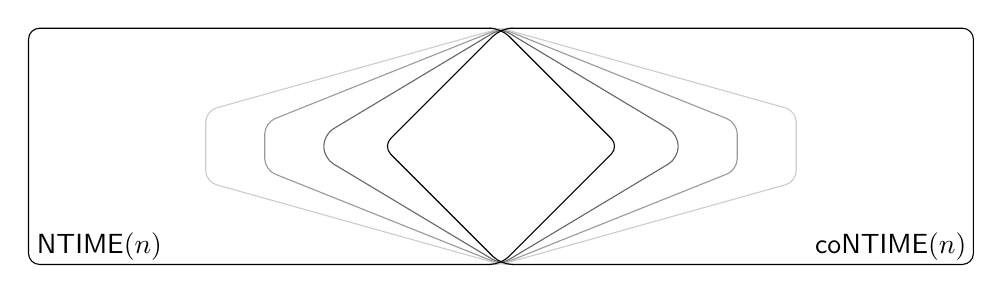
\begin{tikzpicture}[scale=3]
\draw[rounded corners, color=black!60] (1.95, 1) -- (2, 1) -- (2.75, 0.55) -- (2.75, 0.45) -- (2, 0) -- (1.95, 0);
\draw[rounded corners, color=black!40] (1.95, 1) -- (2, 1) -- (3, 0.6) -- (3, 0.4) -- (2, 0) -- (1.95, 0);
\draw[rounded corners, color=black!20] (1.95, 1) -- (2, 1) -- (3.25, 0.65) -- (3.25, 0.35) -- (2, 0) -- (1.95, 0);

\draw[rounded corners, color=black!60] (2.05, 1) -- (2, 1) -- (1.25, 0.55) -- (1.25, 0.45) -- (2, 0) -- (2.05, 0);
\draw[rounded corners, color=black!40] (2.05, 1) -- (2, 1) -- (1, 0.6) -- (1, 0.4) -- (2, 0) -- (2.05, 0);
\draw[rounded corners, color=black!20] (2.05, 1) -- (2, 1) -- (0.75, 0.65) -- (0.75, 0.35) -- (2, 0) -- (2.05, 0);

\draw[rounded corners] (0, 0) -- (0, 1) -- (2, 1) -- (2.5, 0.5) -- (2, 0) -- cycle;
\draw[rounded corners] (4, 0) -- (4, 1) -- (2, 1) -- (1.5, 0.5) -- (2, 0) -- cycle;

\node at (0.3, 0.075) {$\NTIME(n)$};
\node at (3.65, 0.075) {$\coNTIME(n)$};
\end{tikzpicture}
\caption{If $\NTIME(n) \cup \coNTIME(n) = \NTIME\bigl(n^2\bigr) \cup \coNTIME\bigl(n^2\bigr)$, then the $\NTIME$ and $\coNTIME$ hierarchies must grow into $\coNTIME(n)$ and $\NTIME(n)$ respectively. The only thing we can say is that at the very least in this scenario the intersection is a strict hierarchy. So it's impossible for both question marks to become equalities.}
\label{fig:unions-equal}
\end{figure}

Finally, a perhaps even more basic consideration: By Theorem~\ref{X} we know that there exist problems in $\interEXP$ that aren't in $\unionP$. So then where are they? Can we actually point out a concrete problem which separates these classes the way we can in the case of $\NP \subsetneq \NEXP$?

\section*{Solutions}

\begin{enumerate}
\item $2^n$ needs to become $2^{2^n}$ throughout.
\item This establishes Theorem~\ref{NP-interEXP}.
\item
\begin{proof}
Suppose
\[
\NP = \coNEXP\,.
\]
Then
\[
\coNP = \NEXP
\]
via symmetry and
\[
\coNEXP = \NEXPEXP
\]
by padding. Consequently,
\[
\NP = \coNEXP = \NEXPEXP
\]
contradicting Theorem~\ref{NDTH}.
\end{proof}
\end{enumerate}

\begin{thebibliography}{3}
\bibitem{cook}
Stephen A. Cook, \textit{A hierarchy for nondeterministic time complexity}, Proceedings of the fourth annual ACM symposium on Theory of computing, STOC '72, pp. 187--192
\bibitem{stanislav}
Žák Stanislav, \textit{A Turing machine time hierarchy}, Theoretical Computer Science, Elsevier Science B.V. 26, Oct. 1983, pp. 327--333
\bibitem{fortnow}
Lance Fortnow, \url{https://blog.computationalcomplexity.org/2002/11/union-of-complexity-classes.html}, 12. Nov. 2002
\end{thebibliography}

\vfill\eject

\end{document}